
%%%%%%%%%%%%%%%%%%%%%%% file typeinst.tex %%%%%%%%%%%%%%%%%%%%%%%%%
%
% This is the LaTeX source for the instructions to authors using
% the LaTeX document class 'llncs.cls' for contributions to
% the Lecture Notes in Computer Sciences series.
% http://www.springer.com/lncs       Springer Heidelberg 2006/05/04
%
% It may be used as a template for your own input - copy it
% to a new file with a new name and use it as the basis
% for your article.
%
% NB: the document class 'llncs' has its own and detailed documentation, see
% ftp://ftp.springer.de/data/pubftp/pub/tex/latex/llncs/latex2e/llncsdoc.pdf
%
%%%%%%%%%%%%%%%%%%%%%%%%%%%%%%%%%%%%%%%%%%%%%%%%%%%%%%%%%%%%%%%%%%%


\documentclass[runningheads,a4paper]{llncs}

\usepackage{amssymb}
\usepackage{amsmath}
\setcounter{tocdepth}{3}
\usepackage{graphicx}
\newtheorem{mydef}{Definition}
\newtheorem{mylemma}{Lemma}
\usepackage{algorithm}
\usepackage[noend]{algpseudocode}


\usepackage{url}
\urldef{\mailsa}\path|{alfred.hofmann, ursula.barth, ingrid.haas, frank.holzwarth,|
\urldef{\mailsb}\path|anna.kramer, leonie.kunz, christine.reiss, nicole.sator,|
\urldef{\mailsc}\path|erika.siebert-cole, peter.strasser, lncs}@springer.com|    
\newcommand{\keywords}[1]{\par\addvspace\baselineskip
\noindent\keywordname\enspace\ignorespaces#1}

\begin{document}

\mainmatter  % start of an individual contribution

% first the title is needed
\title{Identifiyng Inter-Genomic Repeats Using Fast, Approximate Betweenness Centrality}

% a short form should be given in case it is too long for the running head
\titlerunning{Lecture Notes in Computer Science: Authors' Instructions}

% the name(s) of the author(s) follow(s) next
%
% NB: Chinese authors should write their first names(s) in front of
% their surnames. This ensures that the names appear correctly in
% the running heads and the author index.
%
\author{Alfred Hofmann%
\thanks{Please note that the LNCS Editorial assumes that all authors have used
the western naming convention, with given names preceding surnames. This determines
the structure of the names in the running heads and the author index.}%
\and Ursula Barth\and Ingrid Haas\and Frank Holzwarth\and\\
Anna Kramer\and Leonie Kunz\and Christine Rei\ss\and\\
Nicole Sator\and Erika Siebert-Cole\and Peter Stra\ss er}
%
\authorrunning{Lecture Notes in Computer Science: Authors' Instructions}
% (feature abused for this document to repeat the title also on left hand pages)

% the affiliations are given next; don't give your e-mail address
% unless you accept that it will be published
\institute{Springer-Verlag, Computer Science Editorial,\\
Tiergartenstr. 17, 69121 Heidelberg, Germany\\
\mailsa\\
\mailsb\\
\mailsc\\
\url{http://www.springer.com/lncs}}

%
% NB: a more complex sample for affiliations and the mapping to the
% corresponding authors can be found in the file "llncs.dem"
% (search for the string "\mainmatter" where a contribution starts).
% "llncs.dem" accompanies the document class "llncs.cls".
%

\toctitle{Lecture Notes in Computer Science}
\tocauthor{Authors' Instructions}
\maketitle


\begin{abstract}
The abstract should summarize the contents of the paper and should
contain at least 70 and at most 150 words. It should be written using the
\emph{abstract} environment.
\keywords{We would like to encourage you to list your keywords within
the abstract section}
\end{abstract}


\section{Introduction}

Metagenomics is a direct sequencing of DNA from all organisms in an environment without culturing.  It is a culture-independent tool for studying environmental microorganisms. In addition to the information about taxonomic diversity (‘who is there’), metagenomics gives insight into the physiology of the organisms present in the environment (‘what are they doing’), through studying their genes. Two main goals to be achieved with metagenomics are finding new genes with desired biological activity (bioprospecting) and studying environmental microbes without the need to culture them.

Metagenomic data are considerably more complex. The assembly of metagenomic data is complicated due to several reasons. Few of them are: (i) widely different levels of representation for different organisms in a community; (ii) genomic variation between closely related organisms; (iii) conserved genomic regions shared by distantly related organims; and (iv) repetitive sequences within individual genomes. Genomic repeats are the major challenge when assembling isolated genomes and their effect is prominently seen in metagenomic datasets. It has been show by Kingsford et al.\cite{kingsford} that the number of reconstructions grow exponentially with the number of repeats. Therefore it is impossible find one correct solution for assembly. There are several approaches such as \cite{bambus} to find repeats in metagenomic data. The main drawback of these methods is that they do not scale well as number of nodes in assembly graph increase and prove very inefficient as number of nodes reaches to about a million. To tackle this problem, we explore some of the work in social network analysis, particularly in the area of node centrality. We make use of betweenness centrality to find out repeats in assembly graph. 

\section{Related Work}

\subsection*{Betweenness Centrality}
In graph theory and network analysis, indicators of centrality identify the most important vertices within a graph.Several metrics to measure centrality have been proposed. We make use of betweenness centrality. For a particular node, betweenness centrality is equal to the number of shortest paths from all vertices to all others that pass through that node. Formally, for a node $v$, it is defined by following expression:

$$g(v) = \sum_{s \neq t \neq v} \frac{\sigma_{st}(v)}{\sigma_{st}}$$

where $\sigma_{st}$ is the total number of shortest paths from node $s$ to node $t$ and $\sigma_{st}(v)$ is the number of those paths passing through $v$.

Brandes\cite{brandes} gives an exact algorithm for computing betweenness centrality of all the nodes that is based on solving a single source shortest path problem for each node. An SSSP computation from $s$ produces a directed acyclic graph (DAG) encoding all shortest paths starting at $s$. By backward aggregation of counter values, the contributions of these paths to the betweenness counters can be computed in linear time. Brandes algorithm explains how to calculate $\sigma_{st}$ on the fly during shortest path calculations: $\sigma_{ss} = 1$ and for $s \neq t, \sigma_{st} = \sum_{v \in pred(t)} \sigma_{sv}$ where $pred(t)$ is a multiset containing the immediate predecessors of  $t$ in the shortest path DAG. In a subsequent aggregation phase, the nodes are processed in reverse topological order, i.e. by non-decreasing distance from $s$. So we have: 
$$\delta_{s}(v) = \sum_{w \in succ(v)} \frac{\sigma_{sv}}{\sigma_{sw}}(1+\delta_{s}(w))$$

where $\delta_{s}(v) = \frac{\sigma_{st}(v)}{\sigma_{st}}$ and $succ(v)$ is an immediate successor of $v$  in the shortest path DAG.   
This algorithm takes time $\Theta(mn)$ for unit edge weight graphs and $\Theta(mn + n^{2}log(n))$ for weighted graphs. This algorithm does not scale well with large networks with millions of nodes and edges. Bader and Madduri\cite{bader} provide a massively parallel implementation of the exact algorithm. However this approach scales to about a few million nodes. 

\subsection*{Betweenness Centrality Based on Sampling Nodes}
Due to scalability limitations of exact betweenness centrality, several approximation algorithms for betweenness centrality have been proposed. Bader and Pich\cite{bp} provide an approximation algorithm by extrapolating from a subset of $k$ starting nodes called pivots and using same aggregation strategy as exact betweeness algorithm. However, this algorithm overestimates the centrality of some unimportant nodes which lie near pivot. The approximation algorithm proposed in \cite{sanders} comes over this drawback by changing the scheme for aggregating betweenness contributions so that nodes do not get profited just because they are near pivot. They define an estimator for betweenness centrality. This estimator is characterized by a length function $l : E \Rightarrow \mathbb{R}$ on the edges and a scaling function $f : [0,1] \Rightarrow [0,1]$. For a path $P = (e_{1},e_{2}...,e_{k})$ let $l(P) := \sum_{1 \leq i \leq k} l(e_{i})$. Let $n$ be the number of sample nodes chosen from a graph. The algorithm works as follows: In each iteration one of $2n$ shortest path searches is performed with uniform probability $1/2n$. An iteration can be a forward search in $G = (V,E)$ from a pivot $s \in V$ ($|V| = n$) or backward search from a pivot $t \in V$, that is a search from $t$ in $(V,{(v,u) : (u,v) \in E})$. For each shortest path of the form 
$$ P = (\overbrace{s,...,v}^{Q},..,t)$$ 
a scaled contribution is defined as follows:\\

\begin{equation*}
	\delta_{P}(v) := \begin{cases}
					\frac{f(l(Q)/l(P))}{\sigma_{st}} & \text{for a forward search} \\\\
					\frac{1 - f(l(Q)/l(P))}{\sigma_{st}} & \text{for a backward search} 
					\end{cases}
\end{equation*}

Overall, $v$ receives contribution 

$$\delta(v) := \delta_{s}(v) := \sum_{t \in V}\sum \{\delta_{P}(v):  P \in SP_{st}(v)\}$$
due to a forward search, and 

$$\delta(v) := \delta_{t}(v) := \sum_{s \in V}\sum \{\delta_{P}(v):  P \in SP_{st}(v)\}$$
due to a backward search. 

Geisberger et al. \cite{sanders} have shown that $X := 2n\delta(v)$ is an unbiased estimator of centrality of v that is $E(X) := g(v)$. Therefore by averaging $k$ independent runs of this estimator, we get an approximation $\frac{X_{1}+X_{2}+..+X_{k}}{k}$ of the betweenness centrality for node $v$. 

To compute the contributions of nodes to centrality, a modified scheme of Brandes algorithm is used. Contributions are calculated as follows:

$$\delta_{s}(v) = \sum_{w \in succ(v)} \frac{\mu(s,v)}{\mu(s,w)}.\frac{\sigma_{sv}}{\sigma_{sw}}(1+\delta_{s}(w))$$
where $\mu(s,w)$ is the shortest path distance from $s$ to $w$. It uses $\frac{\mu(s,v)}{\mu(s,w)}$ in aggregation instead of $1$ in Brandes algorithm. 

\subsection*{Betweenness Centrality Based on Sampling Shortest Paths}
There  is another approximation algorithm was proposed by Matteo et al. \cite{matteo} based on randomized sampling of shortest paths and offer probabilistic guarantees on the quality of approximation. This algorithm guarantees that all approximate values of betweenness for all vertices are within an additive factor $\epsilon \in (0,1)$ from the real values with probability at least $1-\delta$. To derive bounds on sample size, results from VC dimension\cite{vc} theory are used. The main advantage of this algorithm is that the sample size does not depend on the size of the graph, but only on the maximum number vertices in a shortest path which is called \textit{vertex diameter}.  

The Vapnik-Chernovenkis(VC) dimensions of a class of subset is defined on a set of points is a measure of expressiveness of such class. Given a probability distribution on the set of points, a finite bound on the VC-dimension of the class of subsets implies a bound on the number of random samples required to approximate the probability of each subset in the class with its empirical average. To define this formally, let $D$ be a domain and $R$ be a collection of subsets from $D$. We call $R$ a \textit{range set} on $D$. Given $B \subseteq D$, the projection of $R$ on $B$ is the set of $P_{R}(B) = \{B \cap A : A \in R\}$.We say that the set $B$ is \textit{shattered} by $R$ if $P_{R}(B) = 2^{B}$, where $2^{B}$ is the powerset of $B$.

\begin{mydef}
The \textit{Vapnik-Chervonenkis} (VC) dimension of $R$, denoted as $VC(R)$, is the cardinality of the largest subset of $D$ that is shattered by $R$.
\end{mydef}

It has been shown that if an upper bound to the VC-dimension of $R$ is available, it is possible to build an $\epsilon$-approximation by sampling the points of the domain according to distribution $\phi$.

\begin{mydef}
Let $R$ be a range set on a domain $D$ with VC(R) $\leq d$, and let $\phi$ be a distribution on $D$. Given $\epsilon, \delta \in (0,1)$ let $S$ be a collection of $|S|$ points from $D$ sampled according to $\phi$ with
\begin{equation} \label{sample_size}
|S| = \frac{c}{\epsilon^{2}}(d + ln\frac{1}{\delta})
\end{equation}

where $c$ is a universal positive constant approximated to 0.5. Then $S$ is an $\epsilon$-approximation to $(R,\phi)$ with probability at least $(1-\delta)$.
\end{mydef}

Using these insights from VC-dimensions, we can define a range set on the shortest paths of a graph $G = (V,E)$ and present a tight upper bound to its VC-dimensions. The range set $R_{G}$ is defined on the set $\mathtt{S}_{G}$ of all shortest paths between vertices of $G$. It contains, for each vertex $v \in V$, the set $T_{v}$ of shortest paths that $v$ is internal to: 
$$R_{G} = \{T_{v} : v \in V\}.$$
Let us define for each shortest path $p$, $Int(p)$ be the set of internal vertices on that path.  Let $H(G)$ be the maximum integer $d$ such that there are $h = \left\lfloor{log_{2}(d-2)}\right\rfloor + 1$ shortest paths $\{p_{1},p_{2},....p_{h}\}$
in $\mathtt{S}_{G}$ of size at least $d$ and such that the collection $\{Int(p_{1}),....,Int(p_{h})\}$ is an anti-chain, that is a collection of sets such that for no two sets in it, one is a subset of other. It has been shown that this can be used to provide an upper bound on VC-dimension on set $R_{G}$. So we have:
$$VC(R_{G}) \leq \left\lfloor{log_{2}(H(G) - 2)}\right\rfloor + 1$$
It $VD(G)$ be the vertex diameter of graph G. It can be shown that $H(G) \leq VD(G)$. As calculating exact $H(G)$ value is hard, we can make use of $VD(G)$ to define upper bound on VC-dimension of $R_{G}$ as follows:
$$VC(R_{G}) \leq \left\lfloor{log_{2}(VD(G) - 2)}\right\rfloor + 1$$

The algorithm to calculate approximate betweenness centrality works as follows. For a graph $G(V,E)$, with vertex diameter $VD(G)$, sample size $r$ is estimated as follows:
$$ d = \left\lfloor{log_{2}(VD(G) - 2)}\right\rfloor + 1$$
Substituting this $d$ in equation\ref{sample_size}, we get
\begin{equation} \label{sample_size_algo}
r = \frac{c}{\epsilon^{2}}(\left\lfloor{log_{2}(VD(G) - 2)}\right\rfloor + 1 + ln\frac{1}{\delta})
\end{equation}
This sample size achieves desired accuracy with the desired confidence. The algorithm repeats following steps $r$ times: 1. It samples a pair of $u,v$ of distinct vertices uniformly at random. 2. It computes set $S_{uv}$ or all shortest paths between $u$ and $v$. 3. It selects path $p$ from $S_{uv}$ at random. 4. It increases by $1/r$ the betweenness estimation of each vertex in $Int(p)$. If sampled vertices $u$ and $v$ are not connected, steps 3 and 4 can be skipped. 

There are two crucial things in this algorithm. First is computing approximate vertex diameter. Calculating exact VD(G) will need to solve all pair shortest  path problem. The complexity of this algorithm is $O(V^{2}logV + VE)$ by Johnson's algorithm\cite{johnson} and $\Theta(V^{3})$ by Floyd-Warshall algorithm. This would be very slow. A faster linear time 2-approximation algorithm is proposed in \cite{matteo}. It is as follows:
\begin{itemize}
\item Select $v \in V$ at random
\item Compute shortest path from $v$ to all vertices in $V$
\item Finally take $VD(G)$ be the sum of lengths of two shortest paths with maximum size from $v$ to two distinct nodes $u$ and $w$. 
\end{itemize}

Second is to sample shortest paths. They way a random shortest path from $S_{uv}$ is inspired by Brandes algorithm\cite{brandes}. Assume that $u$ and $v$ are connected. For each vertex $w$, let $P_{u}(w)$ be a subset of neighbors of $w$ which are predecessors of $w$ along the shortest path from $u$ to $w$. Let $p^{*}$ be the sampled shortest path that we build backwards starting from the endpoint $v$ and by adding sampled predecessors before $v$. Initially $p^{*} = {v}$. Starting from $v$, we select it's predecessor $z \in P_{u}(v)$ using weighted random sampling. Each $z \in P_{u}(v)$ has probability $\sigma_{uz}/\sum_{w \in P_{u}(v)}\sigma_{uv} = \sigma_{uz}/\sigma_{uv}$. We add $z$ to $p^{*}$ and repeat this procedure until $z \neq u$. In the end, we have single shortest path sampled from $S_{uv}$. 
 
\begin{algorithm}
\caption{Algorithm to compute approximate betweenness centrality}
\begin {algorithmic}[1]
\State {\textbf{Input}:Graph $G(V,E)$ with $|V| = n,\epsilon,\delta \in (0,1)$}
\State {\textbf{Output}: A set of approximate betweenness centrality for all nodes $v$ in $G$}
\For {$v \in V$}
\State {$b'(v) = 0$}
\EndFor 
\State {$VD(G) \leftarrow \mathtt{getVertexDiameter}(G)$}
\State {$r \leftarrow \frac{c}{\epsilon^{2}}(\left\lfloor{log_{2}(VD(G) - 2)}\right\rfloor + 1 + ln\frac{1}{\delta})$}
\For{$i \leftarrow 1$ to $r$}
\State {$(u,v) = \mathtt{SampleUniformVertexPair(V)}$}
\State {$S_{uv} = \mathtt{ComputeAllShortestPath(u,v)}$}
\If {$S_{uv} \neq \{p_{\phi}\}$}
\State 	{$t \leftarrow v$}
\While {$t \neq u$}
\State {sample $z \in P_{u}(t)$ with probability $\sigma_{uz}/\sigma_{ut}$}
\If {$z \neq u$}
\State {$b'(z) \leftarrow b'(z) + 1/r$}
\EndIf
\State {$t \leftarrow z$}
\EndWhile
\EndIf
\EndFor\\
\Return {$(v,b'(v)) :\forall v \in V$}
\end{algorithmic}
\end{algorithm}

Analysis of this algorithm shows that it offers probabilistic guarantees on the quality of all approximations of the betweenness centrality. Let $b(v)$ be the actual betweenness centrality of node $v$ and $b'(v)$ be the betweenness centrality returned by algorithm 1. Then following lemma holds:

\begin{mylemma}
With probability atleast $1-\delta$, all the approximations computed by the algorithm are within $\epsilon$ from their real value:
$$Pr(\exists v \in V s.t. |b(v) - b'(v)| > \epsilon) < \delta$$
\end{mylemma}

The runtime of this algorithm is dominated by the computation of shortest path at each step which takes time $O(|V| + |E|)$ if graph is unweighted (BFS) and $O(|E| + |V|log|V|)$ othewise (Dijkstra's algorithm). This is multiplied by $r$ for $r$ iterations to obtain final complexity.


\section{Methods}

\subsection*{De Bruijn Graph} 

De Bruijn strings are a type of 'comprehensive' strings. For a given alphabet $\Sigma = \{A,C,T,G\}$ and a length $k$, a de Bruijn string of order $k$ contains as substrings of length $k$ over $\Sigma$. These strings can be represented in a sophisticated way in term of a graph called de Bruijn graph \cite{debruijn}. A de Bruijn graph of order $k$ is a graph that contains all strings of length $k-1$ from a given alphabets as nodes and contains edges between two nodes if the corresponding strings overlap by exactly $k-2$ letters in prefix-suffix manner. In other words, each $k$-mer is represented by two nodes in a graph connected by an edge. 

We modify the de Bruijn graph generated from genomes to identify repeats in a better way. We define \textit{unipaths} as the path of nodes in which the outdegree of first node on the path is $1$ and indegree is greater than $1$, indegree of last node on the path is $1$ and outdegree is greater than $1$ and for all other nodes, both indegree and out degree is exactly $1$. We compress all the unipaths in a graph to represent in a compact way. For all the internal nodes on unipaths, we represent them by a single node with label as the combined label of all nodes. figure\ref{fig:repeatgraph} shows an example of such compression of unipaths in de Bruijn graphs. 

\begin{figure}[htbp]
\centering
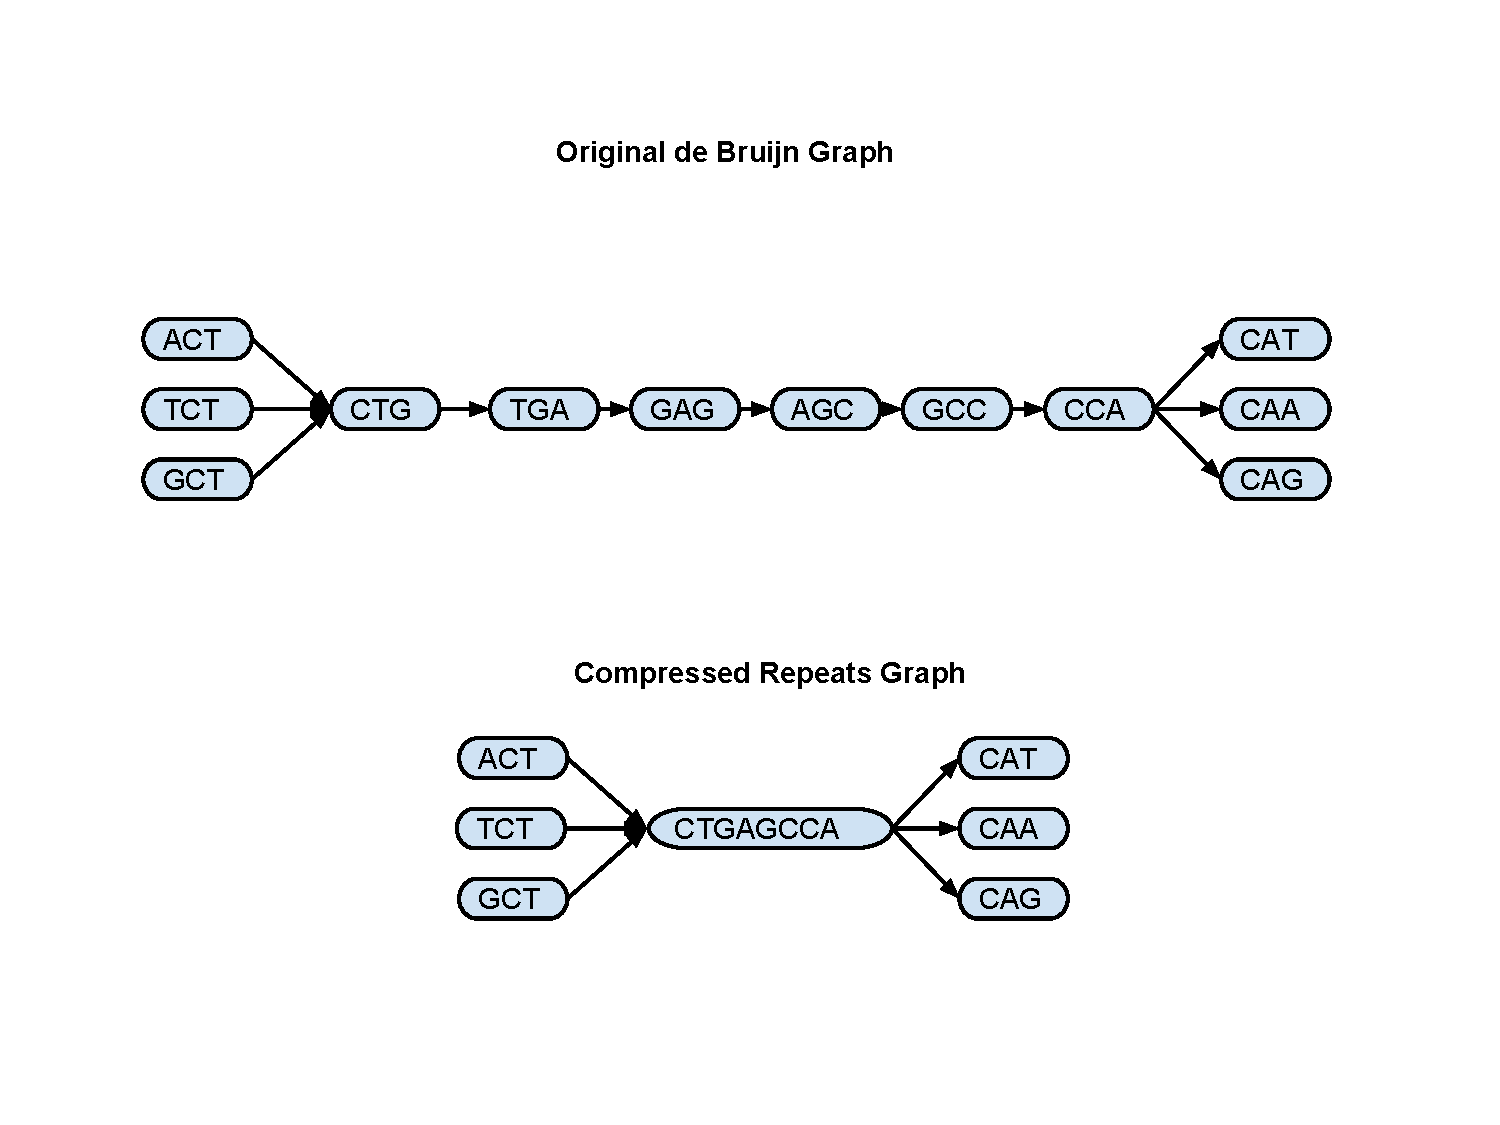
\includegraphics[width = \textwidth]{repeatgraph}
\caption{Example of conversion of de Bruijn graph to Repeats graph}
\label{fig:repeatgraph}
\end{figure}

\subsection*{Networkit}
We investigated the performance of approximate betweenness centrality algorithms on the metagenomic graphs to find inter-genome repeats. We used the implementation in Networkit\cite{networkit} library. It provides implementation for various graph algorithms. We are particularly interested in the implementation of betweenness centrality algorithms. We make use of two approximate betweenness centrality algorithms provided by NetworKit. 

NetworKit provides fast parallel implementation of approximate betweenness centrality algorithm by Matteo et al. \cite{matteo}. The implementation first approximates diameter of of graph. After this, it calculates the number of shortest paths to be sampled. It processes shortest paths in the sample in parallel in multithreaded fashion and then aggregates the centrality scores for each shortest paths once every thread finishes processing of shortest path assigned to it. 

We also investigate the performance of algorithm by Geisberger et al. \cite{sanders}. NetworKit provides single threaded implementation of this algorithm. It first creates a sample of $n$ nodes at random from a given graph. It then runs single source shortest path algorithm for each of those nodes. It calculates the betweenness scores for each node by the modified aggregation scheme proposed in the algorithm. 

Here are few questions we want to investigate based on these algorithms:

\begin{itemize}
\item \textbf{Scalability}: How these algorithms scale on large metagenomic repeats graph? Does parallelized algorithm provides quick results or taking sample of fewer nodes provides quick results?
\item \textbf{Accuracy}: Which of these algorithms provides better accuracy while determining inter-genomic repeats?
\item \textbf{Sample Size}: For the algorithm by Geisberger et al. \cite{sanders}, how should a sample size be defined so that it would produce fast and accurate results? We try to come up with a heuristic to define sample size
\end{itemize}


\subsection*{Cutoff Criteria For Repeats}
To determine which nodes in a graph should be marked as repeats, we define a criteria based on the value of centrality calculated by the algorithm. Let $x$ be the mean of centralities of all the nodes and $\sigma$ be the standard deviation. A node $v$ is marked as repeat only if the following condition holds: $b(v) \geq x + c*\sigma$ where $c$ is a constant and $b(v)$ is betweenness centrality of the node. We set value of $c$ as 3 as it works out the best.

\section{Results} 
We evaluated algorithms for betweenness centrality to find inter-genome repeats on real datasets described above. We use the notion of sensitivity and specificity to define the accuracy of repeat detection. We define following terms:
\begin{itemize}
\item \textbf{True positives:} Number of nodes marked as repeat that is found within at least 2 genomes
\item \textbf{False positives:} Number of nodes marked as repeat that is only repetitive within a single genome
\item \textbf{True negatives:} Number of nodes marked as non-repeat that is only repetitive within a single genome
\item \textbf{False negatives:} Number of nodes marked as non-repeat that is found within at least 2 genomes
\end{itemize}

A good repeat detection should have both good sensitivity and specificity. Sensitivity reflects how many true repeats are detected. Detecting to few repeats can lead to assembly errors in scaffolding. Specificity reflects the false positives. Detecting too many repeats leads to a suboptimal assembly as these contigs do not fully participate in scaffolding. 

\bibliography{manuscript}{}
\bibliographystyle{abbrv}

\end{document}
